
\documentclass[12pt,a4paper]{ctexart}
\usepackage[margin=2.15cm]{geometry}
\usepackage{amsmath,amssymb,mathtools}
\usepackage{graphicx}
\usepackage{enumitem}
\usepackage{booktabs,longtable,array}
\usepackage{tikz}
\usepackage{circuitikz}
\usepackage{xcolor}
\usepackage{hyperref}
\hypersetup{colorlinks=true,linkcolor=black,urlcolor=blue}
\setlength{\parindent}{2em}
\setlength{\parskip}{0.35em}
\setlist[enumerate]{itemsep=0.45em,topsep=0.35em}
\newcommand{\eps}{\varepsilon}
\newcommand{\dif}{\mathop{}\!\mathrm{d}}
\newcommand{\jj}{\mathrm{j}}
\graphicspath{{figures/}}
\begin{document}

\title{\heiti 信号与系统复习：知识点公式表、题目与解析}
\author{}
\date{}


\newpage
\section{核心知识点与公式速查}
\par\bigskip
\noindent\textbf{表1\quad 傅里叶变换常用变换对}
\vspace{0.4em}

\begin{tabular}{p{0.29\textwidth}p{0.64\textwidth}}
\toprule
\textbf{变换对} & \textbf{数学表达式}\\
\midrule
$\displaystyle\delta(t)$ & $1$\\[0.35em]
$\displaystyle1$ & $2\pi\delta(\omega)$\\[0.35em]
$\displaystyle e^{j\omega_0t}$ & $2\pi\delta(\omega-\omega_0)$\\[0.35em]
$\displaystyle\cos\omega_0t$ & $\pi[\delta(\omega-\omega_0)+\delta(\omega+\omega_0)]$\\[0.35em]
$\displaystyle\sin\omega_0t$ & $j\pi[\delta(\omega+\omega_0)-\delta(\omega-\omega_0)]$\\[0.35em]
$\displaystyle\eps(t-a)-\eps(t-b)$ & $\displaystyle\frac{e^{-j\omega a}-e^{-j\omega b}}{j\omega}$\\
\bottomrule
\end{tabular}

\par\bigskip
\noindent\textbf{表2\quad 傅里叶变换基本性质}
\vspace{0.4em}

\begin{tabular}{p{0.29\textwidth}p{0.64\textwidth}}
\toprule
\textbf{性质} & \textbf{数学表达式}\\
\midrule
线性 & $\displaystyle\mathcal F\{af_1(t)+bf_2(t)\}=aF_1(\omega)+bF_2(\omega)$\\[0.35em]
时间移位 & $\displaystyle f(t-t_0)\longleftrightarrow e^{-j\omega t_0}F(\omega)$\\[0.35em]
时域微分 & $\displaystyle\frac{\dif f(t)}{\dif t}\longleftrightarrow j\omega F(\omega)$\\[0.35em]
时域积分 & $\displaystyle\int_{-\infty}^{t}f(\tau)\dif\tau\longleftrightarrow\frac{F(\omega)}{j\omega}+\pi F(0)\delta(\omega)$\\[0.35em]
频域微分 & $\displaystyle(-jt)f(t)\longleftrightarrow\frac{\dif F(\omega)}{\dif\omega}$\\[0.35em]
时域卷积定理 & $\displaystyle f_1(t)*f_2(t)\longleftrightarrow F_1(\omega)F_2(\omega)$\\
\bottomrule
\end{tabular}

\par\bigskip
\noindent\textbf{表3\quad 拉普拉斯变换常用变换对}
\vspace{0.4em}

\begin{tabular}{p{0.29\textwidth}p{0.64\textwidth}}
\toprule
\textbf{变换对} & \textbf{数学表达式}\\
\midrule
$\displaystyle\eps(t)$ & $\displaystyle\frac1s,\quad\operatorname{Re}(s)>0$\\[0.35em]
$\displaystyle e^{-at}\eps(t)$ & $\displaystyle\frac1{s+a},\quad\operatorname{Re}(s)>-a$\\[0.35em]
$\displaystyle\delta(t)$ & $1$\\[0.35em]
$\displaystyle t\eps(t)$ & $\displaystyle\frac1{s^2},\quad\operatorname{Re}(s)>0$\\[0.35em]
$\displaystyle te^{-at}\eps(t)$ & $\displaystyle\frac1{(s+a)^2},\quad\operatorname{Re}(s)>-a$\\
\bottomrule
\end{tabular}

\par\bigskip
\noindent\textbf{表4\quad 拉普拉斯变换基本性质}
\vspace{0.4em}

\begin{tabular}{p{0.29\textwidth}p{0.64\textwidth}}
\toprule
\textbf{性质} & \textbf{数学表达式}\\
\midrule
线性 & $\displaystyle\mathcal L\{af_1(t)+bf_2(t)\}=aF_1(s)+bF_2(s)$\\[0.35em]
延时 & $\displaystyle\mathcal L\{x(t-t_0)\eps(t-t_0)\}=e^{-st_0}X(s)$\\[0.35em]
$s$ 域移位 & $\displaystyle\mathcal L\{e^{-at}f(t)\}=F(s+a)$\\[0.35em]
时域微分 & $\displaystyle\mathcal L\{y'(t)\}=sY(s)-y(0^-)$\\[0.35em]
时域微分(二阶) & $\displaystyle\mathcal L\{y''(t)\}=s^2Y(s)-sy(0^-)-y'(0^-)$\\[0.35em]
时域积分 & $\displaystyle\mathcal L\!\left\{\int_{0^-}^{t}f(\tau)\dif\tau\right\}=\frac{F(s)}{s}$\\[0.35em]
初值定理 & $\displaystyle f(0^+)=\lim_{s\to\infty}sF(s)$\\[0.35em]
终值定理 & $\displaystyle\lim_{t\to\infty}f(t)=\lim_{s\to0}sF(s)$\\[0.35em]
卷积定理 & $\displaystyle f_1(t)*f_2(t)\longleftrightarrow F_1(s)F_2(s)$\\
\bottomrule
\end{tabular}

\par\bigskip
\noindent\textbf{表5\quad 冲激函数的主要性质}
\vspace{0.4em}

\begin{tabular}{p{0.29\textwidth}p{0.64\textwidth}}
\toprule
\textbf{性质} & \textbf{数学表达式}\\
\midrule
抽样性质 & $\displaystyle\int_{t_1}^{t_2}x(t)\delta(t-t_0)\dif t=
\begin{cases}
x(t_0),&t_0\in[t_1,t_2],\\[0.2em]
0,&t_0\notin[t_1,t_2]
\end{cases}$\\[0.8em]
尺度变换 & $\displaystyle\delta(at-b)=\frac1{|a|}\delta\!\left(t-\frac ba\right)\quad(a\ne0)$\\[0.35em]
偶对称 & $\displaystyle\delta(-t)=\delta(t)$\\[0.35em]
与阶跃关系 & $\displaystyle\frac{\dif\eps(t)}{\dif t}=\delta(t)$\\[0.35em]
卷积性质 & $\displaystyle x(t)*\delta(t-t_0)=x(t-t_0)$\\[0.35em]
傅里叶变换 & $\displaystyle\mathcal F\{\delta(t)\}=1$\\[0.35em]
拉普拉斯变换 & $\displaystyle\mathcal L\{\delta(t)\}=1$\\
\bottomrule
\end{tabular}

\par\bigskip
\noindent\textbf{表6\quad 阶跃函数的主要性质}
\vspace{0.4em}

\begin{tabular}{p{0.29\textwidth}p{0.64\textwidth}}
\toprule
\textbf{性质} & \textbf{数学表达式}\\
\midrule
定义 & $\displaystyle\eps(t)=
\begin{cases}
1,&t\ge0,\\[0.2em]
0,&t<0
\end{cases}$\\[0.6em]
截取有限时段 & $\displaystyle x(t)[\eps(t-a)-\eps(t-b)]$ 保留 $x(t)$ 在 $[a,b)$ 的波形\\[0.35em]
与冲激关系 & $\displaystyle\frac{\dif\eps(t)}{\dif t}=\delta(t)$\\[0.35em]
拉普拉斯变换 & $\displaystyle\mathcal L\{\eps(t)\}=\frac1s,\quad\operatorname{Re}(s)>0$\\[0.35em]
卷积性质 & $\displaystyle\eps(t)*h(t)=\int_{-\infty}^{t}h(\tau)\dif\tau$\\[0.35em]
阶跃响应与冲激响应 & $\displaystyle h(t)=\frac{\dif g(t)}{\dif t},\quad g(t)=\int_{-\infty}^{t}h(\tau)\dif\tau$\\
\bottomrule
\end{tabular}

\par\bigskip
\noindent\textbf{表7\quad Z变换常用变换对}
\vspace{0.4em}

\begin{tabular}{p{0.29\textwidth}p{0.64\textwidth}}
\toprule
\textbf{变换对} & \textbf{数学表达式}\\
\midrule
$\displaystyle\delta(k)$ & $1$\\[0.35em]
$\displaystyle\eps(k)$ & $\displaystyle\frac{z}{z-1},\quad |z|>1$\\[0.35em]
$\displaystyle a^k\eps(k)$ & $\displaystyle\frac{z}{z-a},\quad |z|>|a|$\\[0.35em]
$\displaystyle -a^k\eps(-k-1)$ & $\displaystyle\frac{z}{z-a},\quad |z|<|a|$\\[0.35em]
$\displaystyle k\eps(k)$ & $\displaystyle\frac{z}{(z-1)^2},\quad |z|>1$\\[0.35em]
$\displaystyle ka^{k-1}\eps(k)$ & $\displaystyle\frac{z}{(z-a)^2},\quad |z|>|a|$\\
\bottomrule
\end{tabular}

\par\bigskip
\noindent\textbf{表8\quad Z变换基本性质}
\vspace{0.4em}

\begin{tabular}{p{0.29\textwidth}p{0.64\textwidth}}
\toprule
\textbf{性质} & \textbf{数学表达式}\\
\midrule
线性 & $\displaystyle\mathcal Z\{af_1(k)+bf_2(k)\}=aF_1(z)+bF_2(z)$\\[0.35em]
移位（右移） & $\displaystyle\mathcal Z\{x(k-m)\eps(k-m)\}=z^{-m}X(z)$\\[0.35em]
$z$ 域微分 & $\displaystyle\mathcal Z\{k\,x(k)\}=-z\frac{\dif X(z)}{\dif z}$\\[0.35em]
卷积定理 & $\displaystyle x(k)*h(k)\longleftrightarrow X(z)H(z)$\\[0.35em]
系统函数定义 & $\displaystyle H(z)=\frac{Y_{\mathrm{zs}}(z)}{F(z)}$\\[0.35em]
差分方程$\to$系统函数 & $\displaystyle H(z)=\frac{\displaystyle\sum_{m=0}^{M}b_mz^{-m}}{1+\displaystyle\sum_{i=1}^{N}a_iz^{-i}}$\\[0.35em]
离散稳定性 & 因果系统 BIBO 稳定 $\iff$ 全部极点严格在单位圆内\\
\bottomrule
\end{tabular}

\bigskip

\subsection{时域信号、阶跃函数、冲激函数与周期性}
\begin{enumerate}
\item \textbf{阶跃函数截取有限时段。} 对 $a<b$，\(\displaystyle \eps(t-a)-\eps(t-b)\) 只在 $a\le t<b$ 内取 $1$，其他时刻取 $0$。因此，\(\displaystyle x(t)[\eps(t-a)-\eps(t-b)]\) 表示只保留 $x(t)$ 在区间 $[a,b)$ 的波形。这是由波形写出小题中分段余弦信号表达式的直接方法。

\item \textbf{冲激抽样性质。} 若 $t_0$ 在积分区间 $[t_1,t_2]$ 内，则 \(\displaystyle \int_{t_1}^{t_2}x(t)\delta(t-t_0)\dif t=x(t_0)\)；若 $t_0\notin[t_1,t_2]$，则积分结果为 $0$。这解释了积分区间不包含抽样点时，含冲激函数的积分为什么为零。

\item \textbf{冲激函数的尺度与移位。} \(\displaystyle \delta(at-b)=\frac{1}{|a|}\delta\left(t-\frac{b}{a}\right)\;(a\ne0)\)，并且 \(\displaystyle \delta(-t)=\delta(t)\)。例如，\(\displaystyle \delta(3t-3)=\frac13\delta(t-1)\)，\(\displaystyle \delta\left(\frac t2\right)=2\delta(t)\)。

\item \textbf{连续时间正弦信号的周期。} 对 \(\displaystyle A\sin(\omega t+\varphi)\) 或 \(\displaystyle A\cos(\omega t+\varphi)\)，基本周期为 \(\displaystyle T=\frac{2\pi}{|\omega|}\)。若多个非零正弦分量相加，其角频率两两之比均为有理数时才存在有限公共周期；若存在一对角频率之比为无理数，则和信号一般为非周期信号。

\item \textbf{时间变换与支撑区间。} 对 \(\displaystyle g(t)=f(at+b)\)，先令 \(\displaystyle at+b=\tau\)，再把 $f(\tau)$ 的关键时刻 $\tau_i$ 映射为 \(\displaystyle t_i=\frac{\tau_i-b}{a}\)。当 $|a|>1$ 时为时间压缩，$0<|a|<1$ 时为时间扩展，$a<0$ 时还发生时间反折。若已知 $p(t)=f(t+t_0)$，则可用 \(\displaystyle f(t)=p(t-t_0)\) 恢复原信号。

\item \textbf{复合函数求导。} \(\displaystyle \frac{\dif}{\dif t}f(at+b)=a f'(at+b)\)。对分段线性连续信号，导数等于各段斜率；仅当原信号本身出现跳变时，导数中才需要增加相应的冲激项。
\end{enumerate}

\subsection{连续时间 LTI 系统、冲激响应与卷积}
\begin{enumerate}
\item \textbf{系统响应分解。} 全响应满足 \(\displaystyle y(t)=y_{\mathrm{zi}}(t)+y_{\mathrm{zs}}(t)=y_{\mathrm{free}}(t)+y_{\mathrm{forced}}(t)\)。其中，零输入响应 $y_{\mathrm{zi}}(t)$ 仅由初始状态产生；零状态响应 $y_{\mathrm{zs}}(t)$ 仅由外部输入产生。

\item \textbf{冲激响应与卷积。} 对连续时间 LTI 系统，\(\displaystyle y_{\mathrm{zs}}(t)=f(t)*h(t)=\int_{-\infty}^{\infty}f(\tau)h(t-\tau)\dif\tau\)。单位冲激响应 $h(t)$ 描述系统的固有时域特性。

\item \textbf{串联与并联。} 并联系统总冲激响应为各支路冲激响应之和；串联系统总冲激响应为各子系统冲激响应的卷积。常用冲激卷积关系为 \(\displaystyle x(t)*\delta(t-t_0)=x(t-t_0)\)，以及 \(\displaystyle x(t)*[-\delta(t)]=-x(t)\)。

\item \textbf{阶跃响应和冲激响应。} 若阶跃响应为 $g(t)$，则 \(\displaystyle h(t)=\frac{\dif g(t)}{\dif t}\)。反过来，\(\displaystyle g(t)=\int_{-\infty}^{t}h(\tau)\dif\tau\)。

\item \textbf{线性判定。} 线性系统必须同时满足齐次性和可加性，即对任意常数 $\alpha,\beta$，有 \(\displaystyle T\{\alpha x_1+\beta x_2\}=\alpha T\{x_1\}+\beta T\{x_2\}\)。
\end{enumerate}

\subsection{傅里叶级数、傅里叶变换与频谱判定}
\begin{enumerate}
\item \textbf{傅里叶级数的基本角频率。} 周期为 $T$ 的连续时间周期信号，其基本角频率为 \(\displaystyle \omega_0=\frac{2\pi}{T}\)，频谱为位于 $n\omega_0$ 的离散谱线；非周期信号通常对应连续频谱。

\item \textbf{波形对称性。} 若 \(\displaystyle f(-t)=f(t)\)，则 $f(t)$ 为偶函数，傅里叶级数中只含直流分量和余弦项；若 \(\displaystyle f(-t)=-f(t)\)，则为奇函数，只含正弦项。若满足半波对称 \(\displaystyle f(t+T/2)=-f(t)\)，则直流分量和全部偶次谐波均为零。偶函数与半波对称同时满足时，只保留奇次余弦谐波；奇函数与半波对称同时满足时，只保留奇次正弦谐波。

\item \textbf{连续时间傅里叶变换定义。} 采用 \(\displaystyle F(\omega)=\mathcal F\{f(t)\}=\int_{-\infty}^{\infty}f(t)e^{-j\omega t}\dif t\)。线性性质为 \(\displaystyle \mathcal F\{af_1(t)+bf_2(t)\}=aF_1(\omega)+bF_2(\omega)\)。

\item \textbf{常用性质。} 时间移位为 \(\displaystyle f(t-t_0)\longleftrightarrow e^{-j\omega t_0}F(\omega)\)；时域微分为 \(\displaystyle \frac{\dif f(t)}{\dif t}\longleftrightarrow j\omega F(\omega)\)。若 $f(t)$ 在 $\pm\infty$ 处趋于零，且先由 $f'(t)$ 求频谱，则 \(\displaystyle F(\omega)=\frac{\mathcal F\{f'(t)\}}{j\omega}\;(\omega\ne0)\)，再用极限或面积 \(\displaystyle F(0)=\int_{-\infty}^{\infty}f(t)\dif t\) 确定 $\omega=0$ 处的值。

\item \textbf{时域积分性质。} 常规题目中，\(\displaystyle \int_{-\infty}^{t}f(\tau)\dif\tau\longleftrightarrow\frac{F(\omega)}{j\omega}\)。严格形式还应补入直流冲激项：\[\mathcal F\left\{\int_{-\infty}^{t}f(\tau)\dif\tau\right\}=\frac{F(\omega)}{j\omega}+\pi F(0)\delta(\omega).\]

\item \textbf{矩形时窗的变换。} \(\displaystyle \eps(t-a)-\eps(t-b)\longleftrightarrow\frac{e^{-j\omega a}-e^{-j\omega b}}{j\omega}\)。梯形频谱题通常先把梯形求导为若干矩形脉冲之和，再用线性、时移和积分性质求原信号频谱。

\item \textbf{常用变换对。} \[\begin{aligned}
1&\longleftrightarrow 2\pi\delta(\omega),\\
e^{j\omega_0t}&\longleftrightarrow2\pi\delta(\omega-\omega_0),\\
\cos\omega_0t&\longleftrightarrow\pi\bigl[\delta(\omega-\omega_0)+\delta(\omega+\omega_0)\bigr],\\
\sin\omega_0t&\longleftrightarrow j\pi\bigl[\delta(\omega+\omega_0)-\delta(\omega-\omega_0)\bigr],\\
\delta(t)&\longleftrightarrow1.
\end{aligned}\]
\end{enumerate}

\subsection{拉普拉斯变换、微分方程与 $s$ 域电路}
\begin{enumerate}
\item \textbf{拉普拉斯变换与收敛。} 双边拉普拉斯变换为 \(\displaystyle F(s)=\int_{-\infty}^{\infty}f(t)e^{-st}\dif t\)，其中 \(\displaystyle s=\sigma+j\omega\)，且 \(\displaystyle e^{-st}=e^{-\sigma t}e^{-j\omega t}\)。其中 $e^{-\sigma t}$ 是引入的衰减因子，用于使积分满足收敛条件。对右边信号，收敛域通常位于最右极点的右侧。

\item \textbf{常用基本对。} \(\displaystyle \eps(t)\longleftrightarrow\frac1s\)，ROC 为 $\operatorname{Re}(s)>0$；\(\displaystyle e^{-at}\eps(t)\longleftrightarrow\frac1{s+a}\)，ROC 为 $\operatorname{Re}(s)>-a$。

\item \textbf{延时性质。} \(\displaystyle \mathcal L\{x(t-t_0)\eps(t-t_0)\}=e^{-st_0}X(s)\)。特别地，\(\displaystyle e^{-at}\eps(t-t_0)=e^{-at_0}e^{-a(t-t_0)}\eps(t-t_0)\)，从而 \[\mathcal L\{e^{-at}\eps(t-t_0)\}=\frac{e^{-(s+a)t_0}}{s+a},\qquad \operatorname{Re}(s)>-a.\]

\item \textbf{导数的拉普拉斯变换。} 对含初始条件的问题，\(\displaystyle \mathcal L\{y'(t)\}=sY(s)-y(0^-)\)，\(\displaystyle \mathcal L\{y''(t)\}=s^2Y(s)-sy(0^-)-y'(0^-)\)。零初始条件下可简化为 \(\displaystyle \mathcal L\{y^{(n)}(t)\}=s^nY(s)\)。

\item \textbf{系统函数与微分方程。} 零初始条件下，\(\displaystyle H(s)=\frac{Y_{\mathrm{zs}}(s)}{F(s)}\)，即 \(\displaystyle Y_{\mathrm{zs}}(s)=H(s)F(s)\)。若 \(\displaystyle H(s)=\frac{B(s)}{A(s)}\)，则有 \(\displaystyle A(s)Y(s)=B(s)F(s)\)，将 $s$ 替换为微分算子即可得到对应的输入输出微分方程；例如分子含 $s$ 时，对应时域输入的一阶导数项。

\item \textbf{零初始 RLC 电路的阻抗模型。} \(\displaystyle Z_R=R\)，\(\displaystyle Z_C=\frac1{sC}\)，\(\displaystyle Z_L=sL\)。串联电路先用阻抗求电流 \(\displaystyle I(s)=\frac{F(s)}{Z_R+Z_L+Z_C}\)，再由 \(\displaystyle U_C(s)=I(s)Z_C\) 求电容电压，并进行部分分式展开与反变换。

\item \textbf{连续时间稳定性。} 对有理连续时间 LTI 系统，BIBO 稳定的充要条件是全部极点严格位于 $s$ 平面的开左半平面；零点位置不决定 BIBO 稳定性。
\end{enumerate}

\subsection{离散时间信号、卷积和与差分方程}
\begin{enumerate}
\item \textbf{离散阶跃与单位冲激序列。} \(\displaystyle \eps(k)=1\;(k\ge0)\)，\(\displaystyle \eps(k)=0\;(k<0)\)；\(\displaystyle \delta(k)=1\;(k=0)\)，其余 $k$ 取 $0$。移位冲激满足 \(\displaystyle x(k)*\delta(k-k_0)=x(k-k_0)\)。

\item \textbf{离散正弦序列周期条件。} 对 \(\displaystyle x(k)=\sin(\omega_0k+\varphi)\) 或余弦序列，存在正整数 $N$ 和整数 $m$，使 \(\displaystyle N\omega_0=2\pi m\) 时序列才是周期序列；最小正整数 $N$ 为基本周期。多个周期序列相加时，总周期取各基本周期的最小公倍数。

\item \textbf{卷积和。} \(\displaystyle x(k)*h(k)=\sum_{i=-\infty}^{\infty}x(i)h(k-i)\)。当序列由移位冲激的线性组合表示时，可直接利用冲激移位性质逐项卷积；例如 \(\displaystyle \delta(k-m)*\delta(k-n)=\delta(k-m-n)\)。

\item \textbf{单位延时算子。} $E^{-1}$ 表示延时一个采样周期，即 \(\displaystyle E^{-1}x(k)=x(k-1)\)，并有 \(\displaystyle E^{-r}x(k)=x(k-r)\)。读取离散框图时，应先为第一个加法器输出设中间变量 $w(k)$，写出反馈方程，再写输出端前馈方程，最后消去 $w(k)$。

\item \textbf{一般差分方程和系统函数。} 在零初始条件下，若 \[y(k)+\sum_{i=1}^{N}a_i y(k-i)=\sum_{m=0}^{M}b_m f(k-m),\] 则 \[H(z)=\frac{Y(z)}{F(z)}=\frac{\sum_{m=0}^{M}b_mz^{-m}}{1+\sum_{i=1}^{N}a_i z^{-i}}.\] 因此，反馈支路决定分母系数，前馈支路决定分子系数。
\end{enumerate}

\subsection{$Z$ 变换、收敛域、反变换与稳定性}
\begin{enumerate}
\item \textbf{$Z$ 变换定义。} \(\displaystyle X(z)=\mathcal Z\{x(k)\}=\sum_{k=-\infty}^{\infty}x(k)z^{-k}\)。收敛域 ROC 是使该级数收敛的 $z$ 平面区域，且 ROC 不包含极点。

\item \textbf{基本变换对及 ROC。} \[\begin{aligned}
a^k\eps(k)&\longleftrightarrow\frac{z}{z-a},& |z|&>|a|,\\
-a^k\eps(-k-1)&\longleftrightarrow\frac{z}{z-a},& |z|&<|a|.
\end{aligned}\] 因而，对同一个有理式，ROC 在极点外侧对应右边序列，ROC 在极点内侧对应左边序列；ROC 位于两个极点之间时，对不同极点对应的部分必须分别写成右边序列和左边序列。

\item \textbf{求逆 $Z$ 变换。} 常用方法包括部分分式展开法、长除法和围线积分法。部分分式展开后，必须结合给定 ROC 决定每一项究竟对应右边序列还是左边序列，不能只根据代数式直接写出结果。

\item \textbf{极点、零点和稳定性。} 极点由分母为零得到，零点由分子为零得到。离散时间 LTI 系统 BIBO 稳定的条件是单位圆 $|z|=1$ 包含在 ROC 中；对有理因果系统，这等价于全部极点严格位于单位圆内。
\end{enumerate}

\subsection{题目中常用公式与方法映射}
\begin{longtable}{p{0.25\textwidth}p{0.67\textwidth}}
\toprule
\textbf{题型} & \textbf{应调用的公式、知识点或步骤}\\
\midrule
\endfirsthead
\toprule
\textbf{题型} & \textbf{应调用的公式、知识点或步骤}\\
\midrule
\endhead
由波形写阶跃表达式 & 先确定信号非零区间，再写成 \(\displaystyle x(t)[\eps(t-a)-\eps(t-b)]\)；由峰值、过零点或相邻极值判断正弦/余弦的角频率和相位。\\
含冲激函数的积分 & 先检查抽样点是否落在积分区间内；再用 \(\displaystyle \delta(at-b)=\frac1{|a|}\delta\left(t-\frac ba\right)\) 化为标准形式，最后代入被抽样函数。\\
周期判断题 & 单个正弦信号用 \(\displaystyle T=2\pi/|\omega|\)；和信号需要存在公共周期，等价于角频率之比为有理数。\\
时域变换与微分综合题 & 已知 $f(t+t_0)$ 时先恢复 $f(t)$；对 \(\displaystyle f(at+b)\) 映射关键时刻，再按 \(\displaystyle \frac{\dif}{\dif t}f(at+b)=af'(at+b)\) 求导。\\
系统结构与冲激响应综合题 & 并联系统相加、串联系统卷积；使用 \(\displaystyle x(t)*\delta(t-t_0)=x(t-t_0)\) 完成冲激移位。\\
梯形信号频谱综合题 & 先求 $f'(t)$ 并写成矩形脉冲之和；对矩形使用 \(\displaystyle \frac{e^{-j\omega a}-e^{-j\omega b}}{j\omega}\)，最后用 \(\displaystyle F(\omega)=\mathcal F\{f'(t)\}/(j\omega)\) 还原。\\
RLC 零状态响应 & 在 $s$ 域取 \(\displaystyle Z_R=R,\ Z_L=sL,\ Z_C=1/(sC)\)，求 \(\displaystyle I(s)\) 后乘 $Z_C$ 得 $U_C(s)$，再部分分式反变换。\\
含初始条件的连续系统综合题 & 先由 $H(s)=B(s)/A(s)$ 写微分方程；零输入响应使用 \(\displaystyle \mathcal L\{y'\},\mathcal L\{y''\}\) 中的初值项；零状态响应用 \(\displaystyle Y_{\mathrm{zs}}(s)=H(s)F(s)\)，最后两者相加。\\
离散卷积题 & 写卷积和，或把各序列拆为移位冲激的线性组合，使用 \(\displaystyle \delta(k-m)*\delta(k-n)=\delta(k-m-n)\) 合并同类项。\\
离散框图差分方程 & 每个 $E^{-1}$ 对应一个单位延时；先列 $w(k)$ 的反馈式，再列 $y(k)$ 的前馈式，消去 $w(k)$。\\
$Z$ 反变换与收敛域 & 部分分式展开后，对每一个极点结合 ROC 选择右边序列或左边序列；ROC 在极点外、内、之间分别对应不同的时域表示。\\
\bottomrule
\end{longtable}

\newpage
\section{综合题：题目与解析}

\subsection{题 1：时域变换与微分}
\paragraph{题目}
已知信号 $f(t+1)$ 的波形如图，试画出 \(\displaystyle \frac{\dif}{\dif t}\left[f\left(\frac{t}{2}-1\right)\right]\) 的波形。
\begin{center}
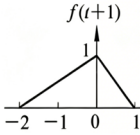
\includegraphics[width=0.36\textwidth]{big_q1_given_signal.png}
\end{center}

\paragraph{解析}
由图可得 $f(t)$ 的支撑区间为 $[-1,2]$，峰值出现在 $t=1$。令 \(\displaystyle g(t)=f\left(\frac t2-1\right)\)。
把 $f(t-1)$ 在时间轴上扩展 2 倍，可得
\[
g(t)=
\begin{cases}
\dfrac{t}{4},&0\le t<4,\\[0.6em]
3-\dfrac{t}{2},&4\le t<6,\\[0.6em]
0,&\text{其他}.
\end{cases}
\]
因此
\[
\boxed{
g'(t)=
\begin{cases}
\dfrac14,&0<t<4,\\[0.4em]
-\dfrac12,&4<t<6,\\[0.4em]
0,&\text{其他}.
\end{cases}}
\]
$g(t)$ 在 $t=0,4,6$ 连续，因此导数中没有冲激项。

\textbf{涉及知识点与公式：}
\begin{itemize}
    \item \textbf{时间变换与支撑区间（第1节第5条）：}由 $f(t+1)$ 恢复 $f(t)$ 波形，再映射 $g(t)=f\!\left(\frac t2-1\right)$ 的关键时间点。当 $|a|>1$ 时压缩，$0<|a|<1$ 时扩展。
    \item \textbf{复合函数求导（第1节第6条）：}$\displaystyle \frac{\mathrm d}{\mathrm d t}f(at+b)=a f'(at+b)$。分段线性信号的导数为各段斜率；仅当原信号出现跳变时导数中才需要增加冲激项。
\end{itemize}

\subsection{题 2：并联--串联系统的冲激响应}
\paragraph{题目}
已知 \(\displaystyle h_1(t)=\eps(t),\ h_2(t)=\delta(t-1),\ h_3(t)=-\delta(t)\)，系统结构如图，求总冲激响应。
\begin{center}
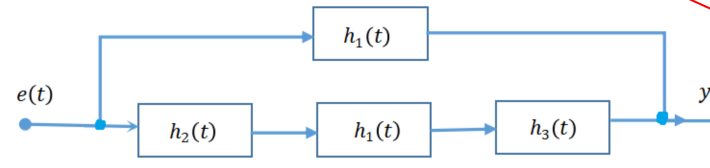
\includegraphics[width=0.88\textwidth]{big_q2_system_block.png}
\end{center}

\paragraph{解析}
上支路只有 $h_1(t)$；下支路为 $h_2(t)$、$h_1(t)$、$h_3(t)$ 串联。因此 \(\displaystyle h(t)=h_1(t)+h_2(t)*h_1(t)*h_3(t)\)。
利用冲激函数的移位、卷积和倒相性质：
\[
h_2*h_1*h_3
=\delta(t-1)*\eps(t)*[-\delta(t)]
=-\eps(t-1).
\]
故
\[
\boxed{h(t)=\eps(t)-\eps(t-1).}
\]

\textbf{涉及知识点与公式：}
\begin{itemize}
    \item \textbf{串联与并联系统（第2节第3条）：}并联总响应为各支路响应之和；串联总响应为各子系统冲激响应的卷积。
    \item \textbf{冲激卷积关系：}$x(t)*\delta(t-t_0)=x(t-t_0)$，$x(t)*[-\delta(t)]=-x(t)$。
\end{itemize}

\subsection{题 3：利用积分性质求梯形信号频谱}
\paragraph{题目}
利用傅里叶变换的积分性质，求下列梯形信号 $f(t)$ 的频谱。
\begin{center}
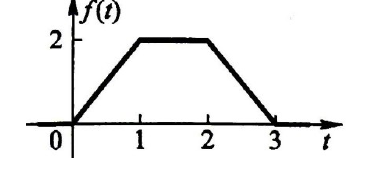
\includegraphics[width=0.38\textwidth]{big_q3_trapezoid.png}
\end{center}

\paragraph{解析}
\textbf{思路：}先对 $f(t)$ 求导得到矩形脉冲组合 $f'(t)$，求出 $f'(t)$ 的频谱，再利用时域积分性质由 $\mathcal F\{f'(t)\}$ 还原 $F(\omega)$。

先求导。由图知
\[
f'(t)=
\begin{cases}
2,&0<t<1,\\
0,&1<t<2,\\
-2,&2<t<3,\\
0,&\text{其他},
\end{cases}
\]
亦可写为 \(\displaystyle f'(t)=2[\eps(t)-\eps(t-1)]-2[\eps(t-2)-\eps(t-3)]\)。

对 $f'(t)$ 作傅里叶变换：
\begin{align*}
\mathcal F\{f'(t)\}
&=2\int_0^1e^{-j\omega t}\dif t
-2\int_2^3e^{-j\omega t}\dif t\\
&=\frac{2}{j\omega}
\left(1-e^{-j\omega}-e^{-j2\omega}+e^{-j3\omega}\right).
\end{align*}

由于 $f(t)=\displaystyle\int_{-\infty}^{t}f'(\tau)\dif\tau$，由\textbf{时域积分性质} $\displaystyle\int_{-\infty}^{t}g(\tau)\dif\tau\longleftrightarrow\frac{G(\omega)}{j\omega}+\pi G(0)\delta(\omega)$，取 $g(t)=f'(t)$，注意 $f'(t)$ 的直流分量 $F_{f'}(0)=\int_{-\infty}^{\infty}f'(t)\dif t=0$（正负面积抵消），故 $\delta$ 项为零，得
\[
\boxed{
F(\omega)=\frac{\mathcal F\{f'(t)\}}{j\omega}
=\frac{2}{(j\omega)^2}
\left(1-e^{-j\omega}-e^{-j2\omega}+e^{-j3\omega}\right).}
\]
等价的三角形式为
\[
\boxed{
F(\omega)=
\frac{8e^{-j\frac{3\omega}{2}}
\sin\frac{\omega}{2}\sin\omega}{\omega^2}.}
\]
在 $\omega=0$ 处取极限，得 $F(0)=4$，正好等于梯形面积。

\textbf{涉及知识点与公式：}
\begin{itemize}
    \item \textbf{时域积分性质（第3节第5条）：}$\displaystyle\int_{-\infty}^{t}g(\tau)\dif\tau\longleftrightarrow\frac{G(\omega)}{j\omega}+\pi G(0)\delta(\omega)$。本题核心，先微分后积分还原。
    \item \textbf{矩形时窗的变换（第3节第6条）：}$\eps(t-a)-\eps(t-b)\longleftrightarrow \dfrac{e^{-j\omega a}-e^{-j\omega b}}{j\omega}$，用于求 $f'(t)$ 的频谱。
\end{itemize}

\subsection{题 4：RLC 零状态响应}
\paragraph{题目}
如图串联 RLC 电路，$R=5\,\Omega$，$L=1\,\mathrm H$，$C=\frac16\,\mathrm F$，零初始条件下输入 $f(t)=12\eps(t)\,\mathrm V$，求 $u_C(t)$。
\begin{center}
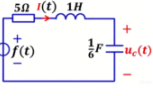
\includegraphics[width=0.25\textwidth]{big_q4_rlc_circuit.png}
\end{center}

\paragraph{解析}
元件阻抗为 \(\displaystyle Z_R=5,\ Z_L=s,\ Z_C=\frac{6}{s}\)。总阻抗为 \(\displaystyle Z(s)=5+s+\frac6s=\frac{s^2+5s+6}{s}\)。输入变换为 $F(s)=12/s$，故 \(\displaystyle I(s)=\frac{F(s)}{Z(s)}\)。
电容电压为
\begin{align*}
U_C(s)
&=I(s)\frac6s\\
&=\frac{12}{s}\cdot\frac{6}{s^2+5s+6}\\
&=\frac{12}{s}-\frac{36}{s+2}+\frac{24}{s+3}.
\end{align*}
因此
\[
\boxed{
u_C(t)=\left(12-36e^{-2t}+24e^{-3t}\right)\eps(t)\ \mathrm V.}
\]

\textbf{涉及知识点与公式：}
\begin{itemize}
    \item \textbf{零初始 RLC 电路 $s$ 域模型（第4节第6条）：}$Z_R=R$，$Z_C=\dfrac1{sC}$，$Z_L=sL$，串联求 $I(s)=\dfrac{F(s)}{Z_R+Z_L+Z_C}$，再由 $U_C(s)=I(s)Z_C$ 得电容电压。
    \item \textbf{常用基本对（第4节第2条）：}$\eps(t)\longleftrightarrow\dfrac1s$，$e^{-at}\eps(t)\longleftrightarrow\dfrac1{s+a}$。配合部分分式展开完成反变换。
    \item \textbf{延时性质（第4节第3条）：}$\mathcal L\{x(t-t_0)\eps(t-t_0)\}=e^{-st_0}X(s)$。
\end{itemize}

\subsection{题 5：由系统函数求微分方程和全响应}
\paragraph{题目}
已知 \(\displaystyle f(t)=e^{-t}\eps(t)\)，\(\displaystyle y(0^-)=1,\ y'(0^-)=2\)，\(\displaystyle H(s)=\frac{3s+1}{s^2+5s+6}\)。求微分方程、零输入响应、零状态响应和全响应。

\paragraph{解析}
由 \(\displaystyle H(s)=\frac{Y_{\mathrm{zs}}(s)}{F(s)}=\frac{3s+1}{s^2+5s+6}\) 可得零初始时的微分方程
\[
\boxed{y''(t)+5y'(t)+6y(t)=3f'(t)+f(t).}
\]
考虑初始条件，对上述方程作拉普拉斯变换：
\[
Y(s)=\underbrace{\frac{s+7}{s^2+5s+6}}_{Y_{\mathrm{zi}}(s)}
+\underbrace{\frac{3s+1}{s^2+5s+6}F(s)}_{Y_{\mathrm{zs}}(s)}.
\]

\textbf{零输入响应：}
\[
Y_{\mathrm{zi}}(s)
=\frac{s+7}{(s+2)(s+3)}
=\frac5{s+2}-\frac4{s+3},
\]
\[
\boxed{
y_{\mathrm{zi}}(t)=\left(5e^{-2t}-4e^{-3t}\right)\eps(t).}
\]

\textbf{零状态响应：} 由于 $F(s)=1/(s+1)$，
\[
Y_{\mathrm{zs}}(s)
=\frac{3s+1}{(s+1)(s+2)(s+3)}
=-\frac1{s+1}+\frac5{s+2}-\frac4{s+3},
\]
\[
\boxed{
y_{\mathrm{zs}}(t)=\left(-e^{-t}+5e^{-2t}-4e^{-3t}\right)\eps(t).}
\]

\textbf{全响应：}
\[
\boxed{
y(t)=\left(-e^{-t}+10e^{-2t}-8e^{-3t}\right)\eps(t).}
\]

\textbf{涉及知识点与公式：}
\begin{itemize}
    \item \textbf{系统函数与微分方程（第4节第5条）：}$H(s)=\dfrac{Y_{\mathrm{zs}}(s)}{F(s)}=\dfrac{B(s)}{A(s)}$，将 $s$ 替换为微分算子得到微分方程；分子含 $s$ 对应输入导数项。
    \item \textbf{导数的拉普拉斯变换（第4节第4条）：}$\mathcal L\{y'(t)\}=sY(s)-y(0^-)$，$\mathcal L\{y''(t)\}=s^2Y(s)-sy(0^-)-y'(0^-)$，用于引入初始条件。
    \item \textbf{系统响应分解（第2节第1条）：}$y(t)=y_{\mathrm{zi}}(t)+y_{\mathrm{zs}}(t)$，分别由初始状态和外部输入产生。
    \item \textbf{部分分式展开与常用基本对：}$\dfrac1{s+a}\longleftrightarrow e^{-at}\eps(t)$。
\end{itemize}

\subsection{题 6：离散卷积和的移位}
\paragraph{题目}
已知 \(\displaystyle f_1(k)=2^{-(k+1)}\eps(k+1)\)，\(\displaystyle f_2(k)=\eps(k-2)\)，求 $f_1(k)*f_2(k)$。

\paragraph{解析}
先定义未移位卷积 \(\displaystyle y_1(k)=2^{-k}\eps(k)*\eps(k)\)。
按卷积和定义，
\begin{align*}
y_1(k)
&=\sum_{i=-\infty}^{\infty}2^{-i}\eps(i)\eps(k-i)\\
&=\sum_{i=0}^{k}2^{-i}\\
&=\left(2-2^{-k}\right)\eps(k).
\end{align*}
又 \(\displaystyle f_1(k)=\left[2^{-k}\eps(k)\right]_{k\mapsto k+1}\)，\(\displaystyle f_2(k)=\left[\eps(k)\right]_{k\mapsto k-2}\)。由卷积的移位性质，\(\displaystyle f_1(k)*f_2(k)=y_1(k+1-2)=y_1(k-1)\)。
故
\[
\boxed{
f_1(k)*f_2(k)=
\left[2-2^{-(k-1)}\right]\eps(k-1).}
\]

\textbf{涉及知识点与公式：}
\begin{itemize}
    \item \textbf{卷积和（第5节第3条）：}$x(k)*h(k)=\displaystyle\sum_{i=-\infty}^{\infty}x(i)h(k-i)$。当序列可写作移位冲激的线性组合时，利用 $\delta(k-m)*\delta(k-n)=\delta(k-m-n)$ 逐项卷积。
    \item \textbf{卷积的移位性质：}$[x(k-m)]*[h(k-n)]=y(k-m-n)$，其中 $y(k)=x(k)*h(k)$。
    \item \textbf{等比数列求和公式：}$\displaystyle\sum_{i=0}^{k}a^{-i}=\frac{1-a^{-(k+1)}}{1-a^{-1}}$。
\end{itemize}

\subsection{题 7：收敛域不同的 $Z$ 反变换}
\paragraph{题目}
已知 \(\displaystyle F(z)=\frac{3z^2}{(z+1)(z-2)}\)，分别求 $|z|>2$、$|z|<1$、$1<|z|<2$ 时的反变换。

\paragraph{解析}
先展开：\(\displaystyle F(z)=\frac{z}{z+1}+2\frac{z}{z-2}\)。
利用
\[
\frac{z}{z-a}\longleftrightarrow
\begin{cases}
a^k\eps(k),&|z|>|a|,\\
-a^k\eps(-k-1),&|z|<|a|.
\end{cases}
\]

\textbf{(1) $|z|>2$：} 两项均为右边序列，
\[
\boxed{
f(k)=\left[(-1)^k+2^{k+1}\right]\eps(k).}
\]

\textbf{(2) $|z|<1$：} 两项均为左边序列，
\[
\boxed{
f(k)=-\left[(-1)^k+2^{k+1}\right]\eps(-k-1).}
\]

\textbf{(3) $1<|z|<2$：} 第一项右边序列，第二项左边序列，
\[
\boxed{
f(k)=(-1)^k\eps(k)-2^{k+1}\eps(-k-1).}
\]

\textbf{涉及知识点与公式：}
\begin{itemize}
    \item \textbf{基本 $Z$ 变换对及 ROC（第6节第2条）：}$a^k\eps(k)\longleftrightarrow \dfrac{z}{z-a},\ |z|>|a|$（右边序列），$-a^k\eps(-k-1)\longleftrightarrow \dfrac{z}{z-a},\ |z|<|a|$（左边序列）。
    \item \textbf{ROC 决定序列类型：}部分分式展开后，每个极点必须结合所在 ROC 判断对应右边还是左边序列；ROC 在极点外侧 $\to$ 右边序列，内侧 $\to$ 左边序列，两极之间 $\to$ 不同极点分别对应左右序列。
\end{itemize}

\newpage
\section{小题：题目、答案与解析}

\subsection{时域信号、冲激函数与周期性}

\begin{enumerate}[label=\arabic*.]
\item \textbf{题目：}写出如图所示信号 $h(t)$ 的表达式。
\begin{center}
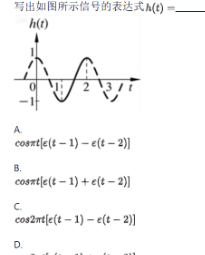
\includegraphics[width=0.29\textwidth]{small_time_q1_signal.png}
\end{center}
\begin{enumerate}[label=\Alph*.]
\item $\cos\pi t[\eps(t-1)-\eps(t-2)]$
\item $\cos\pi t[\eps(t-1)+\eps(t-2)]$
\item $\cos2\pi t[\eps(t-1)-\eps(t-2)]$
\item $\cos2\pi t[\eps(t-1)+\eps(t-2)]$
\end{enumerate}
\textbf{答案：A。}\par
\textbf{解析：} $\eps(t-1)-\eps(t-2)$ 将信号截取在 $1\le t<2$；图中该段为 $\cos\pi t$，故选 A。\\
\textbf{公式依据：}阶跃函数截取有限时段——$\displaystyle x(t)[\eps(t-a)-\eps(t-b)]$ 保留 $x(t)$ 在 $[a,b)$ 波形（第1节第1条）。

\item \textbf{题目：}写出如图所示信号 \(\displaystyle f(t)\) 的表达式。
\begin{center}
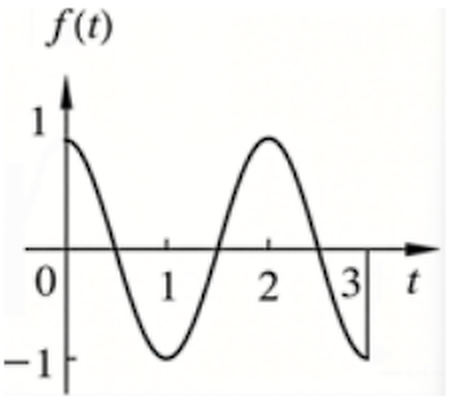
\includegraphics[width=0.29\textwidth]{small_time_q2_signal.png}
\end{center}
\begin{enumerate}[label=\Alph*.]
\item \(\displaystyle \cos\pi t[\eps(t)-\eps(t-2)]\)
\item \(\displaystyle \cos\pi t[\eps(t)-\eps(t-3)]\)
\item \(\displaystyle \cos2\pi t[\eps(t-1)-\eps(t-2)]\)
\item \(\displaystyle \cos2\pi t[\eps(t-1)-\eps(t-3)]\)
\end{enumerate}
\textbf{答案：B。}\par
\textbf{解析：}由波形可知，信号在 \(\displaystyle 0\le t<3\) 时为 \(\displaystyle \cos\pi t\)，其余时刻为零。因此 \(\displaystyle f(t)=\cos\pi t[\eps(t)-\eps(t-3)]\)，故选 B。\\
\textbf{公式依据：}阶跃函数截取有限时段——同上题（第1节第1条）；周期 $\displaystyle T=\frac{2\pi}{|\omega|}$，图中 $\cos\pi t$ 周期为 $2$（第1节第4条）。

\item \textbf{题目：}\(\displaystyle \int_{-\infty}^{\infty} e^{-(t-1)}\delta(t-1)\dif t=\underline{\hspace{1.5cm}}\)。
\textbf{答案：$1$。}\par
\textbf{解析：}\(\displaystyle e^{-(t-1)}\big|_{t=1}=e^0=1\)。\\
\textbf{公式依据：}冲激抽样性质——$\displaystyle\int_{t_1}^{t_2}x(t)\delta(t-t_0)\dif t=x(t_0)$，当 $t_0$ 在积分区间内（第1节第2条）。

\item \textbf{题目：}\(\displaystyle \int_{-\infty}^{\infty}(2t^2+t-5)\delta(3-t)\dif t=\underline{\hspace{1.5cm}}\)。
\textbf{答案：$16$。}\par
\textbf{解析：} $\delta(3-t)=\delta(t-3)$，故 \(\displaystyle 2(3)^2+3-5=16\)。\\
\textbf{公式依据：}冲激抽样性质（第1节第2条）；$\delta(-t)=\delta(t)$ 偶对称性。

\item \textbf{题目：}\(\displaystyle \int_{-\infty}^{\infty} e^{t-1}\delta(3t-3)\dif t=\underline{\hspace{1.5cm}}\)。
\textbf{答案：$\dfrac13$。}\par
\textbf{解析：}\(\displaystyle \delta(3t-3)=\frac13\delta(t-1)\)，所以 \(\displaystyle \int e^{t-1}\delta(3t-3)\dif t=\frac13e^{1-1}=\frac13\)。\\
\textbf{公式依据：}冲激函数的尺度与移位——$\displaystyle\delta(at-b)=\frac1{|a|}\delta\!\left(t-\frac ba\right)$（第1节第3条）。

\item \textbf{题目：}\(\displaystyle \int_{-5}^{5}\left(t^2+t+1\right)\delta\left(\frac{t}{2}\right)\dif t=\underline{\hspace{1.5cm}}\)。
\textbf{答案：$2$。}\par
\textbf{解析：}由冲激函数的尺度性质，\(\displaystyle \delta\left(\frac{t}{2}\right)=2\delta(t)\)。因此 \(\displaystyle \int_{-5}^{5}\left(t^2+t+1\right)\delta\left(\frac{t}{2}\right)\dif t=2\left(t^2+t+1\right)\big|_{t=0}=2\)。\\
\textbf{公式依据：}冲激尺度性质——$\displaystyle\delta\!\left(\frac t2\right)=2\delta(t)$（第1节第3条），然后代入抽样点 $t=0$。

\item \textbf{题目：}\(\displaystyle \int_{-1}^{1}\left(t^2+t-1\right)\delta(t-2)\dif t=\underline{\hspace{1.5cm}}\)。
\textbf{答案：$0$。}\par
\textbf{解析：}冲激函数的抽样点在 $t=2$，但 $2\notin[-1,1]$，故积分区间内没有冲激作用点，因此积分结果为 $0$。\\
\textbf{公式依据：}冲激抽样性质——抽样点不在积分区间内时积分结果为 $0$（第1节第2条）。

\item \textbf{题目：}两个连续周期信号之和不一定是周期信号。（对/错）\par
\textbf{答案：对。}\par
\textbf{解析：}两个周期信号之和只有在它们周期之比为有理数时才一定仍为周期信号；若周期之比为无理数，则和信号一般不是周期信号，因此题述正确。\\
\textbf{公式依据：}多个周期信号相加时，角频率之比全为有理数才存在公共周期（第1节第4条）。

\item \textbf{题目：}$f(t)=4\sin2t+5\cos\pi t$ 的周期是 $2\pi$。（对/错）\par
\textbf{答案：错。}\par
\textbf{解析：}$4\sin2t$ 的周期为 $\pi$，$5\cos\pi t$ 的周期为 $2$。若存在公共周期 $T$，则 $T=n\pi=2m$。由于 $\pi$ 为无理数，不存在正的公共周期，故该和信号不是周期信号。\\
\textbf{公式依据：}周期公式 $\displaystyle T=\frac{2\pi}{|\omega|}$（第1节第4条）；两角频率之比 $\dfrac{2}{\pi}$ 为无理数 $\Rightarrow$ 非周期。

\item \textbf{题目：}$f(t)=A\sin t+B\cos(\sqrt2\,t)$ 是非周期信号。（对/错）\par
\textbf{答案：对（通常假定 $A,B\ne0$）。}\par
\textbf{解析：}两个角频率之比为 $1/\sqrt2$，是无理数，因此无有限公共周期。\\
\textbf{公式依据：}角频率之比为无理数时和信号为非周期信号（第1节第4条）。
\end{enumerate}

\subsection{连续时间系统与卷积}

\begin{enumerate}[label=\arabic*.]
\item \textbf{题目：}仅由系统初始状态引起的响应称为\underline{\hspace{1.5cm}}响应。\par
\textbf{答案：零输入响应。}\par
\textbf{解析：}令外部输入为零，仅保留初始储能或初始状态带来的响应。\\
\textbf{公式依据：}系统响应分解——$y(t)=y_{\mathrm{zi}}(t)+y_{\mathrm{zs}}(t)$（第2节第1条）。

\item \textbf{题目：}仅由系统外部激励信号引起的响应称为\underline{\hspace{1.5cm}}响应。\par
\textbf{答案：零状态响应。}\par
\textbf{解析：}令所有初始条件为零，仅保留外部输入所引起的响应。\\
\textbf{公式依据：}系统响应分解——$y(t)=y_{\mathrm{zi}}(t)+y_{\mathrm{zs}}(t)$（第2节第1条）。

\item \textbf{题目：}单位冲激响应 $h(t)$ 描述的是系统的\underline{\hspace{1.5cm}}。
\begin{enumerate}[label=\Alph*.]
\item 外部激励特性
\item 初始状态
\item 固有时域特性
\item 稳态输出
\end{enumerate}
\textbf{答案：A。}\par
\textbf{解析：}$h(t)$ 是系统在零初始条件下对 $\delta(t)$ 的输出，是描述输入--输出关系的外部激励特性。\\
\textbf{公式依据：}冲激响应 $h(t)$ 定义——系统在零初始条件下对 $\delta(t)$ 的输出（第2节第2条）。

\item \textbf{题目：}连续时间系统零状态响应的求解公式是\underline{\hspace{1.5cm}}。
\begin{enumerate}[label=\Alph*.]
\item $y(t)=f(t)+h(t)$
\item $y(t)=f(t)-h(t)$
\item $y(t)=f(t)\times h(t)$
\item $y(t)=f(t)*h(t)$
\end{enumerate}
\textbf{答案：D。}\par
\textbf{解析：}LTI 系统零状态响应由输入与冲激响应的卷积给出。\\
\textbf{公式依据：}$y_{\mathrm{zs}}(t)=f(t)*h(t)=\int_{-\infty}^{\infty}f(\tau)h(t-\tau)\dif\tau$（第2节第2条）。

\item \textbf{题目：}连续时间系统的系统响应划分错误的是\underline{\hspace{1.5cm}}。
\begin{enumerate}[label=\Alph*.]
\item 全响应 $=$ 零输入响应 $+$ 零状态响应
\item 全响应 $=$ 冲激响应 $+$ 阶跃响应
\item 全响应 $=$ 暂态响应 $+$ 稳态响应
\item 全响应 $=$ 自由响应 $+$ 强迫响应
\end{enumerate}
\textbf{答案：B。}\par
\textbf{解析：}冲激响应与阶跃响应是系统特性，不是给定输入与初始条件下全响应的两种互补划分。\\
\textbf{公式依据：}全响应 $=$ 零输入 $+$ 零状态 $=$ 自由 $+$ 强迫 $=$ 暂态 $+$ 稳态（第2节第1条）。

\item \textbf{题目：}已知 LTI 系统的阶跃响应为 $g(t)$，求 冲激响应$h(t)$。\par
\textbf{答案：}
\[
\boxed{h(t)=\frac{\dif g(t)}{\dif t}.}
\]
\textbf{解析：}$g(t)=\eps(t)*h(t)$；对两边求导即可。\\
\textbf{公式依据：}阶跃响应与冲激响应关系——$h(t)=\dfrac{\dif g(t)}{\dif t}$（第2节第4条）。

\item \textbf{题目：}零输入响应为自由响应；零状态响应为强迫响应。（对/错）\par
\textbf{答案：对。}\par
\textbf{解析：}零输入响应只由初始条件决定，属于自由响应；零状态响应由外部输入驱动，属于强迫响应。\\
\textbf{公式依据：}$y(t)=y_{\mathrm{zi}}(t)+y_{\mathrm{zs}}(t)=y_{\mathrm{free}}(t)+y_{\mathrm{forced}}(t)$（第2节第1条）。

\item \textbf{题目：}线性特性指的是齐次性和可加性。（对/错）\par
\textbf{答案：对。}\par
\textbf{解析：}线性定义为 \(\displaystyle T\{a x_1+b x_2\}=aT\{x_1\}+bT\{x_2\}\)。\\
\textbf{公式依据：}线性系统判定——同时满足齐次性和可加性（第2节第5条）。
\end{enumerate}

\subsection{傅里叶变换}

\noindent\textbf{前置概念：}
\begin{itemize}
    \item \textbf{直流分量}（$n=0$）：傅里叶级数中的常数项 $\displaystyle\frac{a_0}{2}$，代表信号的均值或平均值。半波对称信号 $f(t+T/2)=-f(t)$ 的直流分量为零。
    \item \textbf{偶次谐波分量}（$n=2,4,6,\dots$）：频率为基波频率 $\omega_0$ 的偶数倍（$2\omega_0,4\omega_0,\dots$）的分量。半波对称信号的偶次谐波全部为零。
    \item \textbf{奇次谐波分量}（$n=1,3,5,\dots$）：频率为基波频率 $\omega_0$ 的奇数倍（$\omega_0,3\omega_0,5\omega_0,\dots$）的分量。
\end{itemize}

\noindent\textbf{谐波成分的快速判定：}
\begin{itemize}
    \item 将波形\textbf{右移半个周期} $f(t+T/2)$，若与原波形 $f(t)$ \textbf{完全重合} $\Longrightarrow$ 信号含有\textbf{直流分量和偶次谐波}。
    \item 将波形\textbf{右移半个周期再上下翻转} $-$ $f(t+T/2)$，若与原波形 $f(t)$ \textbf{完全重合}（即 $f(t+T/2)=-f(t)$，半波对称）$\Longrightarrow$ 信号\textbf{只含奇次谐波}（直流和偶次均为零）。
\end{itemize}

\noindent\textbf{正弦/余弦分量的判定（奇偶性）：}
\begin{itemize}
    \item \textbf{偶函数} $f(-t)=f(t)$ $\Longrightarrow$ 傅里叶级数中\textbf{只含余弦分量}（含直流项 $a_0/2$）。
    \item \textbf{奇函数} $f(-t)=-f(t)$ $\Longrightarrow$ 傅里叶级数中\textbf{只含正弦分量}（直流 $a_0=0$）。
    \item 结合半波对称：偶函数 $+$ 半波对称 $\Longrightarrow$ \textbf{只含奇次余弦分量}；奇函数 $+$ 半波对称 $\Longrightarrow$ \textbf{只含奇次正弦分量}。
\end{itemize}

\begin{enumerate}[label=\arabic*.]
\item \textbf{题目：}周期信号如图所示，其傅里叶级数展开式中包含何种分量？
\begin{center}
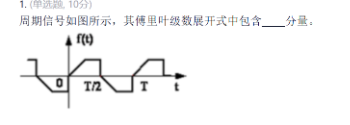
\includegraphics[width=0.48\textwidth]{fourier_q1_waveform.png}
\end{center}
\begin{enumerate}[label=\Alph*.]
\item 只含有奇次谐波的余弦分量
\item 只含有直流和偶次谐波分量
\item 只含有奇次谐波分量
\item 只含有偶次谐波分量
\end{enumerate}
\textbf{答案：C。}\par
\textbf{解析：}图中波形具有半波对称性 $f(t+T/2)=-f(t)$，因此直流分量和偶次谐波均为零；但仅由半波对称性不能断定只含正弦或只含余弦项，故选 C。\\
\textbf{公式依据：}半波对称——$f(t+T/2)=-f(t)$ 时直流和偶次谐波为零（第3节第2条）。

\item \textbf{题目：}周期信号如图所示，其傅里叶级数展开式中包含何种分量？
\begin{center}
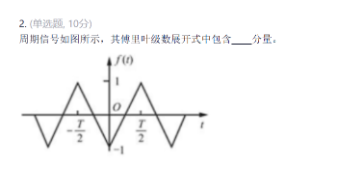
\includegraphics[width=0.44\textwidth]{fourier_q2_waveform.png}
\end{center}
\begin{enumerate}[label=\Alph*.]
\item 只含有奇次谐波的余弦分量
\item 只含有直流和偶次谐波分量
\item 只含有奇次谐波分量
\item 只含有偶次谐波分量
\end{enumerate}
\textbf{答案：A。}\par
\textbf{解析：}该波形既为偶函数，又具有半波对称性；偶函数只含余弦项，半波对称性消去直流和偶次谐波，故只余奇次余弦项。\\
\textbf{公式依据：}偶函数只含余弦项，半波对称消去偶次谐波（第3节第2条）。

\item \textbf{题目：}时域微分对应频域何种运算？
\begin{enumerate}[label=\Alph*.]
\item 乘以 $j\omega$
\item 除以 $j\omega$
\item 乘以 $js$
\item 除以 $js$
\end{enumerate}
\textbf{答案：A。}\par
\textbf{解析：}$\mathcal F\{f'(t)\}=j\omega F(\omega)$。\\
\textbf{公式依据：}时域微分性质——$\dfrac{\mathrm d f(t)}{\mathrm d t}\longleftrightarrow j\omega F(\omega)$（第3节第4条）。

\item \textbf{题目：}时域积分对应频域何种运算？
\begin{enumerate}[label=\Alph*.]
\item 乘以 $j\omega$
\item 除以 $j\omega$
\item 乘以 $js$
\item 除以 $js$
\end{enumerate}
\textbf{答案：B。}\par
\textbf{解析：}基础题中按 $F(\omega)/(j\omega)$ 处理；严格形式需补充直流冲激项。\\
\textbf{公式依据：}时域积分性质——$\displaystyle\int_{-\infty}^{t}f(\tau)\dif\tau\longleftrightarrow\frac{F(\omega)}{j\omega}$（第3节第5条）。

\item \textbf{题目：}下列傅里叶变换错误的是哪一项？
\begin{enumerate}[label=\Alph*.]
\item $1\longleftrightarrow2\pi\delta(\omega)$
\item $e^{j\omega_0t}\longleftrightarrow2\pi\delta(\omega-\omega_0)$
\item $\cos(\omega_0t)\longleftrightarrow\pi[\delta(\omega+\omega_0)+\delta(\omega-\omega_0)]$
\item $\sin(\omega_0t)\longleftrightarrow j\pi[\delta(\omega+\omega_0)+\delta(\omega-\omega_0)]$
\end{enumerate}
\textbf{答案：D。}\par
\textbf{解析：}\(\displaystyle \sin(\omega_0t)\longleftrightarrow j\pi[\delta(\omega+\omega_0)-\delta(\omega-\omega_0)]\)，两项之间应为减号。\\
\textbf{公式依据：}常用变换对——$\cos\omega_0t\longleftrightarrow\pi[\delta(\omega-\omega_0)+\delta(\omega+\omega_0)]$，$\sin\omega_0t\longleftrightarrow j\pi[\delta(\omega+\omega_0)-\delta(\omega-\omega_0)]$（第3节第7条）。

\item \textbf{题目：}下列关于傅里叶变换的说法正确的是哪一项？
\begin{enumerate}[label=\Alph*.]
\item 仅适用于周期信号
\item 仅适用于非周期信号
\item 适用于满足狄利克雷条件的周期、非周期信号
\item 所有信号均可做傅里叶变换
\end{enumerate}
\textbf{答案：C。}\par
\textbf{解析：}非周期信号可作傅里叶变换；周期信号可用冲激谱或广义函数意义下的傅里叶变换描述，通常要求满足相应条件。\\
\textbf{公式依据：}傅里叶变换定义——$F(\omega)=\int_{-\infty}^{\infty}f(t)e^{-j\omega t}\dif t$，适用于满足狄利克雷条件的信号（第3节第3条）。

\item \textbf{题目：}下列信号中，频谱为离散谱的是哪一项？
\begin{enumerate}[label=\Alph*.]
\item 周期矩形脉冲信号
\item 单个矩形脉冲信号
\end{enumerate}
\textbf{答案：A。}\par
\textbf{解析：}连续时间周期信号对应离散谱；单个有限时宽矩形脉冲对应连续频谱。\\
\textbf{公式依据：}周期信号的 FS 系数位于 $n\omega_0$ 的离散谱线（第3节第1条）。

\item \textbf{题目：}$\mathcal F\{\delta(t)\}=\underline{\hspace{1.5cm}}$。\par
\textbf{答案：$1$。}\par
\textbf{解析：}\(\displaystyle \mathcal F\{\delta(t)\}=\int_{-\infty}^{\infty}\delta(t)e^{-j\omega t}\dif t=1\)。\\
\textbf{公式依据：}常用变换对——$\delta(t)\longleftrightarrow1$（第3节第7条）。
\end{enumerate}

\subsection{拉普拉斯变换与连续系统的 $s$ 域分析}

\begin{enumerate}[label=\arabic*.]
\item \textbf{题目：}拉普拉斯变换中引入的衰减因子为哪一项？
\begin{enumerate}[label=\Alph*.]
\item $e^{-\sigma t}$
\item $e^{\sigma t}$
\item $e^{-j\omega t}$
\item $e^{j\omega t}$
\end{enumerate}
\textbf{答案：A。}\par
\textbf{解析：}$e^{-st}=e^{-\sigma t}e^{-j\omega t}$，其中 $e^{-\sigma t}$ 负责收敛。\\
\textbf{公式依据：}拉普拉斯变换定义——$F(s)=\int_{-\infty}^{\infty}f(t)e^{-st}\dif t$，$e^{-st}=e^{-\sigma t}e^{-j\omega t}$，$e^{-\sigma t}$ 为衰减因子（第4节第1条）。

\item \textbf{题目：}$f(t)=\eps(t-2)$ 的单边拉普拉斯变换及收敛域为哪一项？
\begin{enumerate}[label=\Alph*.]
\item $\dfrac1s e^{-2s},\ \sigma<0$
\item $\dfrac1s e^{-2s},\ \sigma>0$
\item $\dfrac1s e^{2s},\ \sigma<0$
\item $\dfrac1s e^{2s},\ \sigma>0$
\end{enumerate}
\textbf{答案：B。}\par
\textbf{解析：}\(\displaystyle \mathcal L\{\eps(t-2)\}=e^{-2s}\frac1s,\quad \operatorname{Re}(s)>0\)。\\
\textbf{公式依据：}延时性质——$\mathcal L\{x(t-t_0)\eps(t-t_0)\}=e^{-st_0}X(s)$（第4节第3条）；$\eps(t)\longleftrightarrow\frac1s$（第4节第2条）。

\item \textbf{题目：}$f(t)=4e^{-2t}\eps(t-3)$ 的单边拉普拉斯变换及收敛域为哪一项？
\begin{enumerate}[label=\Alph*.]
\item $\dfrac4{s-2}e^{-3(s-2)},\ \sigma>2$
\item $\dfrac4{s-2}e^{3(s-2)},\ \sigma>2$
\item $\dfrac4{s+2}e^{-3(s+2)},\ \sigma>-2$
\item $\dfrac4{s+2}e^{3(s+2)},\ \sigma>-2$
\end{enumerate}
\textbf{答案：C。}\par
\textbf{解析：}\(\displaystyle 4e^{-2t}\eps(t-3)=4e^{-6}e^{-2(t-3)}\eps(t-3)\)，故 \(\displaystyle F(s)=\frac4{s+2}e^{-3(s+2)},\ \operatorname{Re}(s)>-2\)。\\
\textbf{公式依据：}延时性质与指数衰减——$e^{-at}\eps(t-t_0)=e^{-at_0}e^{-a(t-t_0)}\eps(t-t_0)$，$\mathcal L\{e^{-at}\eps(t)\}=\frac1{s+a}$（第4节第2、3条）。

\item \textbf{题目：}若 \(\displaystyle H(s)=\frac{3s}{s^2+5s+6}\)，其对应微分方程为哪一项？
\begin{enumerate}[label=\Alph*.]
\item $y''-5y'-6y=3f$
\item $y''-5y'-6y=3f'$
\item $y''+5y'+6y=3f$
\item $y''+5y'+6y=3f'$
\end{enumerate}
\textbf{答案：D。}\par
\textbf{解析：}零初始条件下 \(\displaystyle (s^2+5s+6)Y(s)=3sF(s)\)，回到时域即 \(\displaystyle y''+5y'+6y=3f'\)。\\
\textbf{公式依据：}系统函数与微分方程——$H(s)=\frac{B(s)}{A(s)}$，$A(s)Y(s)=B(s)F(s)$，$s$ 替换为微分算子（第4节第5条）。

\item \textbf{题目：}RLC 电路零状态响应下的 $s$ 域元件模型分别为何？
\begin{enumerate}[label=\Alph*.]
\item $R,\ C,\ L$
\item $R,\ sC,\ sL$
\item $R,\ \dfrac1{sC},\ sL$
\item $R,\ sC,\ \dfrac1{sL}$
\end{enumerate}
\textbf{答案：C。}\par
\textbf{解析：}由 $i_C=C\,\dif u_C/\dif t$ 和 $u_L=L\,\dif i_L/\dif t$ 可得零初始阻抗模型。\\
\textbf{公式依据：}$s$ 域元件模型——$Z_R=R$，$Z_C=\dfrac1{sC}$，$Z_L=sL$（第4节第6条）。

\item \textbf{题目：}极点 $p_1=-2,p_2=-5$、零点 $z_1=1$ 的连续 LTI 系统稳定。（对/错）\par
\textbf{答案：对。}\par
\textbf{解析：}极点均在左半平面，系统 BIBO 稳定；零点 $z_1=1$ 不影响稳定性。\\
\textbf{公式依据：}连续时间稳定性——BIBO 稳定 $\iff$ 全部极点位于开左半 $s$ 平面（第4节第7条）。

\item \textbf{题目：}连续 LTI 系统零状态响应满足 $Y_{\mathrm{zs}}(s)=F(s)H(s)$。（对/错）\par
\textbf{答案：对。}\par
\textbf{解析：}这是系统函数定义直接给出的关系。\\
\textbf{公式依据：}$Y_{\mathrm{zs}}(s)=H(s)F(s)$，系统函数定义（第4节第5条）。
\end{enumerate}

\subsection{第五章：离散时间信号与系统}

\begin{enumerate}[label=\arabic*.]
\item \textbf{题目：}\(\displaystyle f(k)=\sin\frac{\pi(k-1)}4\) 的周期为\underline{\hspace{1.5cm}}。\par
\textbf{答案：$8$。}\par
\textbf{解析：}$\omega_0=\pi/4$，令 $N\omega_0=2\pi$，得 $N=8$；相位平移不改变周期。\\
\textbf{公式依据：}离散正弦序列周期条件——$N\omega_0=2\pi m$，最小正整数 $N$ 为基本周期（第5节第2条）。

\item \textbf{题目：}\(\displaystyle f(k)=\sin\frac{2k\pi}{7}+\cos\frac{2k\pi}{3}\) 的周期为\underline{\hspace{1.5cm}}。\par
\textbf{答案：$21$。}\par
\textbf{解析：}两项周期分别为 $7$ 与 $3$，总周期为 \(\displaystyle N=\operatorname{lcm}(7,3)=21\)。\\
\textbf{公式依据：}离散周期——$N\omega_0=2\pi m$ 求每项周期，和信号总周期取各周期的最小公倍数（第5节第2条）。

\item \textbf{题目：}离散时间系统的特点描述错误的是哪一项？
\begin{enumerate}[label=\Alph*.]
\item 自变量取整数
\item 幅值一定是二进制数字
\item 输入为离散序列
\item 输出为离散序列
\end{enumerate}
\textbf{答案：B。}\par
\textbf{解析：}离散时间只约束自变量为离散整数，序列幅值可以是实数、复数或任何离散/连续数值，并非必须二进制。\\
\textbf{公式依据：}离散时间信号定义——自变量 $k$ 取整数，幅值可为任意值（第5节第1条）。

\item \textbf{题目：}列出图示离散时间系统的输入输出差分方程。
\begin{center}
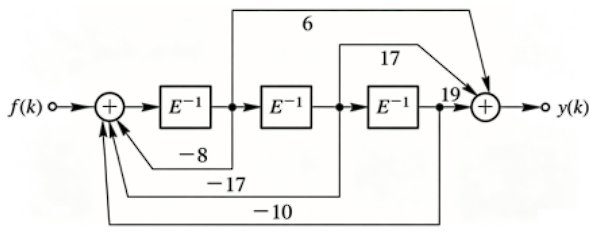
\includegraphics[width=0.86\textwidth]{discrete_q4_block.png}
\end{center}
选项为：
\begin{enumerate}[label=\Alph*.]
\item $y(k)+8y(k-1)+17y(k-2)+10y(k-3)=6f(k-1)+17f(k-2)+19f(k-3)$
\item $y(k)-8y(k-1)-17y(k-2)=6f(k-1)+17f(k-2)+19f(k-3)$
\item $f(k)-8f(k-1)-17f(k-2)=6y(k-1)+17y(k-2)+19y(k-3)$
\item $f(k)+8f(k-1)+17f(k-2)=6y(k-1)+17y(k-2)+19y(k-3)$
\end{enumerate}
\textbf{答案：A。}\par
\textbf{解析：}令第一个加法器输出为 $w(k)$。图中三条反馈支路的系数分别为 $-8$、$-17$、$-10$，故 \(\displaystyle w(k)=f(k)-8w(k-1)-17w(k-2)-10w(k-3)\)。输出端三条前馈支路的系数分别为 $6$、$17$、$19$，故 \(\displaystyle y(k)=6w(k-1)+17w(k-2)+19w(k-3)\)。消去 $w(k)$ 后得到
\[
\boxed{
y(k)+8y(k-1)+17y(k-2)+10y(k-3)
=6f(k-1)+17f(k-2)+19f(k-3).}
\]
\textbf{公式依据：}离散框图——设加法器输出 $w(k)$，反馈支路决定分母（$y$ 侧）系数，前馈支路决定分子（$f$ 侧）系数；$E^{-1}$ 为单位延时算子（第5节第4、5条）。

\item \textbf{题目：}已知 \(\displaystyle f_1(k)=4\delta(k)+3\delta(k-1)+\delta(k-3)\)，\(\displaystyle f_2(k)=3\delta(k)+2\delta(k-1)\)，求 $f_1(k)*f_2(k)$。
\begin{enumerate}[label=\Alph*.]
\item $\{1,3,7,9,2\}$
\item $\{12,17,9,2\}$
\item $\{1,3,7,6,3,2\}$
\item $\{12,17,6,3,2\}$
\end{enumerate}
\textbf{答案：D。}\par
\textbf{解析：}
\[
\begin{aligned}
f_1*f_2
={}&12\delta(k)+17\delta(k-1)+6\delta(k-2)\\
&+3\delta(k-3)+2\delta(k-4).
\end{aligned}
\]
故系数序列为 $\{12,17,6,3,2\}$。\\
\textbf{公式依据：}卷积和——拆为移位冲激的线性组合，利用 $\delta(k-m)*\delta(k-n)=\delta(k-m-n)$ 逐项卷积（第5节第3条）。
\end{enumerate}

\subsection{第七章：$Z$ 变换}

\begin{enumerate}[label=\arabic*.]
\item \textbf{题目：}求逆 $Z$ 变换用方法不包含哪一项？
\begin{enumerate}[label=\Alph*.]
\item 部分分式展开法
\item 长除法
\item 微分法
\item 围线积分法
\end{enumerate}
\textbf{答案：C。}\par
\textbf{解析：}常用反变换方法包括部分分式展开、长除和围线积分；微分法不是本题所列的标准反变换方法。\\
\textbf{公式依据：}求逆 $Z$ 变换——部分分式展开法、长除法、围线积分法（第6节第3条）。

\item \textbf{题目：}\(\displaystyle H(z)=\frac{z}{(z+0.5)(z+0.25)}\) 的极点位置为何？
\begin{enumerate}[label=\Alph*.]
\item $z=0$
\item $z_1=0.5,\ z_2=0.25$
\item $z_1=-0.5,\ z_2=-0.25$
\end{enumerate}
\textbf{答案：C。}\par
\textbf{解析：}令分母为零，即 $z=-0.5$ 或 $z=-0.25$。\\
\textbf{公式依据：}极点由分母为零得到（第6节第4条）。

\item \textbf{题目：}\(\displaystyle y(k)+\frac34y(k-1)+\frac18y(k-2)=f(k)\)。求 $H(z)$ 并判定稳定性。
\begin{enumerate}[label=\Alph*.]
\item $\displaystyle \frac1{1+\frac34z^{-1}+\frac18z^{-2}}$，稳定
\item $\displaystyle \frac1{1-\frac34z^{-1}-\frac18z^{-2}}$，稳定
\item $\displaystyle \frac1{1+\frac34z^{-1}+\frac18z^{-2}}$，不稳定
\item $\displaystyle \frac1{1-\frac34z^{-1}-\frac18z^{-2}}$，不稳定
\end{enumerate}
\textbf{答案：A。}\par
\textbf{解析：}零初始 $Z$ 变换得 \(\displaystyle H(z)=\frac{Y(z)}{F(z)}=\frac1{1+\frac34z^{-1}+\frac18z^{-2}}\)。特征多项式为 \(\displaystyle z^2+\frac34z+\frac18=(z+0.5)(z+0.25)\)，极点模值均小于 1，故系统稳定。\\
\textbf{公式依据：}差分方程与系统函数——$H(z)=\dfrac{\sum b_mz^{-m}}{1+\sum a_i z^{-i}}$（第5节第5条）；离散稳定性——极点全部在单位圆内（第6节第4条）。

\item \textbf{题目：}\(\displaystyle f(k)=2^k\eps(-k-1)\) 的 $Z$ 变换收敛域为 $|z|>2$。（对/错）\par
\textbf{答案：错。}\par
\textbf{解析：}该序列为左边序列，\(\displaystyle 2^k\eps(-k-1)\longleftrightarrow-\frac{z}{z-2},\ |z|<2\)。\\
\textbf{公式依据：}基本 $Z$ 变换对——$a^k\eps(k)\longleftrightarrow\frac{z}{z-a},\ |z|>|a|$（右边）；$-a^k\eps(-k-1)\longleftrightarrow\frac{z}{z-a},\ |z|<|a|$（左边）（第6节第2条）。

\item \textbf{题目：}因果离散系统稳定的充要条件是极点全部在单位圆内。（对/错）\par
\textbf{答案：对（针对有理因果系统）。}\par
\textbf{解析：}因果系统的 ROC 在最外极点之外；BIBO 稳定要求单位圆包含在 ROC 中，因此全部极点必须严格位于单位圆内。\\
\textbf{公式依据：}离散系统稳定性——对有理因果系统，BIBO 稳定 $\iff$ 全部极点严格在单位圆内（第6节第4条）。
\end{enumerate}

\end{document}
